\chapter{Cutting planes for signomial programming }
\label{chap.sig}

\section{Introduction}


In this chapter, we provide a deeper treatment of the \emph{signomial term} $\psi_{\alpha}(x) \deq x^{\alpha} =\prod_{j \in [n]} x_j^{\alpha_j}$, where  the exponent vector $\alpha$ is in $\bR^n$, with respect to convexification and linearization within an sBB algorithm. 

When all the terms in $g$ in \eqref{minlp2} are signomial terms, the problem \eqref{minlp2} falls under the category of signomial programming (SP). In this scenario, we refer to \eqref{minlp2} as the \emph{natural formulation} of SP. The left-hand sides of the constraints in this formulation are referred to as \emph{signomial functions}. The lifted set $\cSl$ in the extended formulation \eqref{minlp3} is called a \emph{signomial lift}. 

Since negative entries may be present in the exponent vector $\alpha$, in general, variables of SP are assumed to be positive. We remark that the  techniques in this chapter can also treat signomial terms in general mixed-integer NLP problems. The point of restriction on  SP over positive variables is simply to make the theoretical treatment more readable and
streamlined.

In the case of SP, LP relaxations can be derived from polyhedral outer approximations of the signomial lift in its extended formulation.
A typical relaxation algorithm for SP involves factoring the signomial term $\psi_{\alpha}(x)$ into the product of $n$ univariate signomial terms $x_i^{\alpha_i}$. Following the factorization, the algorithm proceeds to convexify and linearize the intermediate multilinear term and univariate functions. However, this factorable programming approach can lead to a weak LP relaxation and introduce additional auxiliary variables representing intermediate functions. These issues have been previously discussed in the context of pure multilinear terms \cite{cafieri2010convex, costa2012relaxations, speakman2017quantifying}.


We propose two cutting plane-based relaxation algorithms for SP. In contrast to the conventional factorable programming approach, our method employs a novel reformulation of the signomial lift. We study outer approximations of the following graph of the signomial term:
\begin{equation}
    \cS = \{(x,y): y = x^\alpha\}.
\end{equation}

 We transform each nonlinear equality constraint $y_i = g_i(x) = x^{\alpha^i}$ in \eqref{eq.lift} to an equivalent constraint $ \psi_{\beta}(u) - \psi_{\gamma}(v) = 0$, where $\beta > 0, \gamma>0$, $\max(\norm{\beta}_1, \norm{\gamma}_1)=1$, $u,v$ are disjoint sub-vectors of $(x,y_i)$, and $ \psi_{\beta} , \psi_{\gamma} $ are concave functions. We consider approximating the following set
\begin{equation}
\label{eq.sform}
	\cSt\deq\{(u, v) \in \bR_{+}^{h + \ell}:\, \psi_{\beta}(u) - \psi_{\gamma}(v) \le 0\}.
\end{equation}

Our first cutting plane  algorithm is based on the intersection cut paradigm \cite{conforti2011}. One can approximate  a nonconvex set $\cS$ using its simplicial conic outer approximation. This requires the construction of $\cS$-free sets, which are closed convex sets containing none of the interiors of $\cS$. The main insight about $\cS$-free sets for a nonconvex set $\cS$ is that they provide an explicit and useful description of convex parts of the infeasible space w.r.t.~$\cS$.  

Our second cutting plane algorithm is based on the conventional underestimating and overestimating techniques.  To ensure the convergence of the sBB algorithm, a common assumption for SP is that all variables are bounded. We generate linear underestiamtor (resp. linear overestimator) for $\psi_{\beta}(u)$ (resp. $\psi_{\gamma}(v)$). This yields a convex outer approximation of $\cSt$.


\subsection{Literature review}
 SP finds applications in diverse areas, such as aeronautics \cite{Opgenoord2017},  chemical reactors \cite{Blau1971}, delta-sigma modulator topologies \cite{Harjunkoski1998}, design of heat exchanger networks \cite{Bjork2002}, inductors \cite{Jabr2007}, and trim-loss minimization \cite{Harjunkoski1998}.   

The majority of relaxations for SP are derived from its generalized geometric programming (GPP) formulation,  which is an exponential transformation \cite{duffin1970linearizing}  of its natural formulation. The exponential transformation replaces positive variables $x$ by exponentials $\exp(z)$, where $z$ are real variables. The authors of  \cite{maranas1997global} show that signomial functions in GGP are difference-of-convex (DC) functions. For the signomial function in each constraint of GGP, they  construct linear underestimators of its concave part; the author  of \cite{shen2005linearization} constructs linear underestimators of the whole function via the mean value theorem. The author of \cite{xu2014global} proposes inner approximations  of GGP via the inequality of  arithmetic and geometric means (AM-GM inequality). The authors of \cite{chandrasekaran2016,dressler2022algebraic,murray2021signomial} construct  non-negativity certificates for signomial functions via the AM-GM inequality, and propose a hierarchy of convex relaxations for GGP. Exponential transformations can be combined with other variable transformations, such as  power transformations, and the inverse transformations can be approximated by piece-wise linear functions, see \cite{lin2012range,lundell2013reformulation,lundell2018}.

The solvers \scip \cite{bestuzheva2023global}, \baron \cite{tawarmalani2005polyhedral}, \antigone \cite{Misener2014}, and \miso \cite{misener2012global,Misener2014miso} are capable of solving the natural formulation of SP or its extended formulation within a global $\epsilon$-optimality using the sBB algorithm. Specifically, \miso is a specialized solver for SP that employs exponential transformations of some signomial terms only when necessary.  Due to the following reasons, exponential transformations can complicate general-purpose solvers. First, in certain NLP problems, signomial terms may appear only as a subset of the nonlinear terms of $g(x)$. In such cases, solvers may need to enforce the inverse transformation $x_j = \ln(z_j)$, which requires additional processing for convexification algorithms. Secondly, when dealing with mixed-integer SP, if some variables of $x$ are integers, exponential transformations lead to certain components of $z$ becoming discrete but not necessarily integer. As a result, the sBB algorithm needs to adapt its branching rules.

While considerable attention has been devoted to constructing relaxations for GGP, the literature on relaxations for the extended natural formulation of SP is relatively limited. The convex relaxations employed in the mentioned solvers mainly rely on factorable programming \cite{leonelson, mccormick1976computability}. Since exponential transformations are nonlinear variable transformations, it is impossible to directly apply the relaxations designed for the GGP formulation to the natural formulation.

Numerous research efforts have been dedicated to improving the relaxation techniques for multilinear terms and univariate/bivariate functions commonly used in factorable programming \cite{bao2015global}. Multilinear terms over the unit hypercube  are vertex polyhedral, and  their envelopes over the unit hypercube admit simple extended formulations  \cite{rikun1997convex}. Notably, closed forms for the convex envelopes of bilinear functions \cite{al1983jointly, mccormick1976computability} and trilinear functions \cite{meyer2004trilinear, meyer20042} over hypercubes are well-established. In \cite{sherali1997convex}, the author presents convex envelopes for multilinear functions (sum of multilinear terms) over the unit hypercube and specific discrete sets. For a comprehensive analysis of multilinear term factorization via bilinear terms, we refer to \cite{luedtke2012some, speakman2017quantifying}. Additionally, \cite{cafieri2010convex} offers an in-depth examination of quadrilinear function factorization through bilinear and trilinear terms, while \cite{costa2012relaxations} presents a computational study on extended formulations.

Convexifying univariate/bivariate functions plays an important role in the field of MINLP optimzation. In \cite{liberti2003convex}, convex envelopes for monomials with odd degrees are derived. An approach presented in \cite{locatelli2014convex} enables the evaluation of the convex envelope of a bivariate function over a polytope and separating its supporting hyperplane by solving low-dimensional convex optimization problems. The convex optimization problems are further reduced by solving a Karush-Kuhn-Tucker system \cite{locatelli2018convex}. In \cite{locatelli2016polyhedral}, convex envelopes for bilinear, fractional, and other bivariate functions over a polytope are constructed using a polyhedral subdivision technique. Additionally, \cite{nguyen2018deriving, tawarmalani2013explicit} employ polyhedral subdivision and lift-project methods to derive explicit forms of convex envelopes for various non-convex functions, including a specific subclass of bivariate signomial terms.

Convexifying high-order multivariate functions poses a significant challenge, and the available literature on convex underestimators for trivariate functions is relatively scarce. In \cite{he2021new, he2022tractable}, the authors propose a novel framework for relaxing composite functions in nonlinear programs. Another approach involves using the intersection cut paradigm \cite{conforti2011} to approximate nonconvex functions. This paradigm can generate cutting planes to strengthen LP relaxations of NLP problems. Constructing intersection cuts involves searching for an $\cS$-free set, where $\cS$ represents a nonconvex set defined by nonconvex functions.

The study of intersection cuts originated in the context of NLP \cite{thy1985}. Gomory later introduced the concept of corner polyhedron \cite{gomory1969some}, and intersection cuts were explored in the field of integer programming \cite{balas1971}. The modern definition of intersection cuts for arbitrary sets $\cS$ is from \cite{dey2008, glover1973}. For more comprehensive details, we refer to \cite{andersen2010, basu2010, basu2019, cornuejols2015sufficiency, del2012relaxations, dey2008, richard2010group}. Recent research has revealed $\cS$-free sets for various nonconvex sets encountered in structured NLP problems. Examples include outer product sets \cite{bienstock2019}, sublevel sets of DC functions \cite{serrano2019}, quadratic sets \cite{munoz2020maximal}, and graphs of bilinear terms \cite{fischetti2020}. Intersection cuts  have also been developed for convex mixed-integer NLP problems \cite{andersen2007, belotti2015conic, klnc-karzan2015, kilinc-karzan2016, modaresi2016} and for bilevel programming \cite{fischetti2018}.






\subsection{Contribution}


We give the transformation procedure leading to $\cSt$ and construct $\cSt$-free sets from the transformation. We show that these sets are also signomial-lift-free and maximal in the non-negative orthant. We also discuss the separation of intersection cuts. 

Our second cutting plane algorithm aims at approximating $\cSt$ within a hypercube.  In \Cref{sec.outerforsp}, we provide an extended formulation for the convex envelope of the concave function $\psi_{\beta}$ over the hypercube. This formulation yields a convex outer approximation of $\cSt$, allowing us to generate outer approximation cuts  through projection. We prove that $\psi_{\beta}$ is a supermodular function. For $h=2$, we provide a closed-form expression for its convex envelope by exploiting supermodularity: this allows us to remove the projection step.


About the computational part of this study, we note that signomials are one of the four main types of nonlinearity occurring in the mixed-integer NLP library (\minlplib) \cite{minlpsurveyAN, minlplib}. Our relaxation approach does not require factorization or introduce intermediate functions, making the implementation of the proposed cutting planes within the general-purpose solver \scip straightforward.



\subsection{Notation}
 For a vector $x \in \bR^n$, given $J \subseteq [n]$, $x_J = (x_j)_{j \in J}$ denotes  the sub-vector  formed by entries indexed by $J$.  Given a differentiable function $f$, for a $\relx{x} \in \dom(f)$, $\nabla{f}(\relx{x})$  denotes the gradient of $f$ at $\relx{x}$ and  
\begin{equation}
    \lin{f}{\relx{x}}(x) := f(\relx{x}) + \nabla f(\relx{x}) \cdot(x - \relx{x}). \label{def.Xi}
\end{equation}

The word \textit{linearization} has two different meanings in mathematical programming: (i) a symbolic one, which entails the replacement of all occurrences of nonlinear term $\tau(x)$ with a new variable $t$, followed by the addition of a new constraint $t=\tau(x)$ in a formulation --- this is also called a ``lifting''; (ii) an analytic one, which involves the replacement of a convex nonlinear constraint with an affine subspace tangent to the nonlinear surface at a given point. All mentions of linearization in the rest of this chapter refer to the second meaning.


\subsection{Outline of the chapter}
In \Cref{sec.icforsp}, we construct several families of $\cS$-free sets, study their maximalities, and derive intersection cuts. In \Cref{sec.outerforsp}, we construct a nonlinear relaxation of the signomial term set, and derive outer approximation cuts through projection. In \Cref{sec.comp},
we perform computational tests on instances from \minlplib and observe  improvements to \scip's default settings due to the proposed valid inequalities.


\section{Signomial-lift-free sets and intersection cuts}
\label{sec.icforsp}
In this section, we  construct  (maximal) signomial-lift-free sets and generate intersection cuts for SP.  

\subsection{Signomial-lift-free and signomial-term-free sets}
\label{sec.siliftfree}

We introduce and study formulations of signomial term sets. We transform signomial term sets into DCC sets. Furthermore, we construct  signomial-term-free sets and lift them to signomial-lift-free sets. The maximality of these sets is investigated, and a comparison is carried out between signomial-term-free sets derived from different DCC formulations.


We consider an $n$-variate signomial term $\psi_{\alpha}(x)$ arising in the extended formulation \eqref{minlp3} of SP.
The exponent vector $\alpha$ may contain negative/zero/positive entries. We extract  two sub-vectors $\alpha^-$ and $\alpha^+$ from $\alpha$ such that $\alpha^- < 0 \in \bR^{h'}$ and $\alpha^+ > 0 \in \bR^{\ell'}$, and let $x_- \in \bR^{h'}$ and  $x_+ \in \bR^{\ell'}$ be the corresponding sub-vectors of $x$. Entries $x_j$ with $\alpha_j = 0$ are excluded from consideration, and so $h' + \ell'$ may be smaller than $n$. Since $\psi_{\alpha}(x)$ only depends on $x_-$ and $x_+$, it can be represented in the form of $x_{-}^{\alpha^-} x_{+}^{\alpha^+}$ of lower order. Then, a \emph{signomial term set} is defined as  epigraph or hypograph of $x_{-}^{\alpha^-}  x_{+}^{\alpha^+}$:
\begin{equation}
	\label{eq.sigset}
  \cSt = \{(x_-,x_+, t) \in \bR_{++}^{h' + \ell'+1}: t  \lesseqgtr x_{-}^{\alpha^-}  x_{+}^{\alpha^+} \}.
\end{equation}


We first give DCC reformulations of  signomial term sets.
Let $\lessgtr$ denote  $<$ or $>$. The interior of $\cSt$ in \eqref{eq.sigset} is
 \begin{equation*}
   \inter(\cSt) = \{(x_-,x_+, t) \in \bR_{++}^{h' + \ell'+1} : t \lessgtr x_{-}^{\alpha^-}  x_{+}^{\alpha^+} \}.
\end{equation*}
Reorganizing the signomial terms and taking the closure of the set, we recover
\begin{equation*}
  	\cSt =\{ (x_-,x_+, t) \in \bR_{+}^{h' + \ell'+1}:  t x_-^{-\alpha^-} \lesseqgtr x_+^{\alpha^+}\}.
\end{equation*}


Notably, the exponents associated with signomial terms on both sides are now strictly positive. Let $\bR_{++}$ denote the positive orthant. Let $u \deq (t,x_-), v \deq x_+$, let $h \deq h'+1$, and let $\ell \deq \ell'$. Then, $\psi_{\beta'}(u)=t x_-^{-\alpha^-}$ and $ \psi_{\gamma'}(v)=x_+^{\alpha^+}$, where \(\beta'\deq(1, -\alpha^-) \in \bR_{++}^h\) and \(\gamma' \deq \alpha^+  \in \bR_{++}^\ell\).  After the change of variables, the set  admits the following form:
\begin{equation}
\label{eq.form1}
	\cSt =  \{(u, v) \in \bR_{+}^{h + \ell}:\, \psi_{\beta'}(u) \lesseqgtr \psi_{\gamma'}(v)\},
\end{equation}
where $\lesseqgtr$ denote  $\le$ or $\ge$.

The formulation \eqref{eq.form1} exhibits symmetry between $u$ and $v$.  We can therefore consider w.l.o.g.~the inequality ``$\le$'' throughout the subsequent analysis.
Since the signomial terms $\psi_{\beta'}(u), \psi_{\gamma'}(v)$
are non-negative over $\bR_{+}^h, \bR_{+}^\ell$, we can take any positive power $\eta \in \bR_{++}$ on both sides of \eqref{eq.form1}.  Finally, the signomial  term set in \eqref{eq.sigset} admits the following form:
\begin{equation}
\label{eq.form2}
	\cSt =  \{(u, v) \in \bR_{+}^{h + \ell}:\, \psi_{\beta}(u) - \psi_{\gamma}(v) \le 0\},
\end{equation}
where $\beta \deq \eta \beta'$, and $\gamma \deq \eta \gamma'$.

A signomial term $\psi_{\alpha}(x)$ is said to be a \emph{power function} if $\alpha \ge 0$, and $\lVert \alpha \rVert_1 \le 1$. According to \cite{aps2018mosek,chares2009cones}, power functions are concave over the non-negative orthant; if additionally $\lVert \alpha \rVert_1 = 1$, $\psi_{\alpha}(x)$ is positive  homogeneous of degree 1. Through an appropriate scaling of the parameter $\eta$, we obtain a family of DCC reformulations \eqref{eq.form2} of signomial term sets. We let $\cG\deq  \bR_{+}^{h + \ell}$, and use the reverse-linearization technique  to construct signomial-term-free sets. We recall that the definition of the operator $\Xi$ is given in Eq.~\eqref{def.Xi}.
\begin{proposition}
\label{prop.maxsig}
Let $\max(\lVert \beta \rVert_1, \lVert \gamma \rVert_1 ) \le  1$. For any $\relx{v} \in \bR^{\ell}_{++}$, \begin{equation}
\label{eq.sigfree}
	\cC \deq  \{(u, v) \in \bR_{+}^h \times \bR^{\ell}:\, \psi_{\beta}(u) - \lin{\psi_{\gamma}}{\relx{v}}(v) \ge 0\}
\end{equation} is a signomial-term-free ($\cSt$-free) set.   If $\max(\lVert \beta \rVert_1, \lVert \gamma \rVert_1 ) = 1$, then $\cC$ is a maximal signomial-term-free set in $\cG$.
 \end{proposition}
 \begin{proof}
Since $ \max(\lVert \beta \rVert_1, \lVert \gamma \rVert_1 ) \le 1 $,  $ \psi_{\beta}(u), \psi_{\gamma}(v)$ are concave. By \Cref{cor.dc2}, $\cC$ is signomial-term-free. If $\max(\lVert \beta \rVert_1, \lVert \gamma \rVert_1 ) = 1$, then  at least one of $\lVert \beta \rVert_1,  \lVert \gamma \rVert_1$ is 1. Therefore, one of $\psi_{\beta}(u), \psi_{\gamma}( v)$ is positive  homogeneous of degree 1.  Moreover, $\psi_{\beta}(u), \psi_{\gamma}( v)$ are both continuously differentiable and positive over positive orthants $\bR^h_{++},\bR^{\ell}_{++}$ (the interiors of their domains). Since $\cG = \dom(\psi_{\beta}) \times  \dom(\psi_{\gamma})$,  by \Cref{thm.max}, $\cC \cap \cG= \{(u, v) \in \cG:\, \psi_{\beta}(u) - \lin{\psi_{\gamma}}{\relx{v}}(v) \ge 0\}$  is  a maximal signomial-term-free set in $\cG$. Therefore, $\cC$ is also a maximal signomial-term-free set in $\cG$.
 \end{proof}
 
Given that $ \max(\lVert \beta \rVert_1, \lVert \gamma \rVert_1 ) = 1$ results in a desirable DDC formulation for the signomial term set, we refer to this formulation as its \emph{normalized DCC formulation}.  Comparing \Cref{prop.maxsig} to \Cref{thm.max}, we extend the domain of $\lin{\psi_{\gamma}}{\relx{v}}(v)$ from $\bR^{\ell}_{+}$ to $\bR^{\ell}$, since it is an affine function. However, the further extension requires a non-trivial concave extension of the power function $\psi_{\beta}$, for which we are unaware of a closed-form expression.

We have reduced the $n$-variate signomial term $\psi_{\alpha}(x)$ to a signomial term $ x_{-}^{\alpha^-}  x_{+}^{\alpha^+}$ of lower order and constructed the corresponding signomial-term-free sets. A similar reduction is observed for $g_i$ to $g'_i$ in \Cref{sec.lift}, where we demonstrate the relationship between  $\cSl$-free sets and  $\epi(g'_i)$-free/$\hyp(g'_i)$-free sets.

Next, we let the lifted set $\cSl$ be the signomial lift,  where all $g_i$ are signomial terms. Each equality constraint $y_i = g_i(x)$ defining the signomial lift is equivalent to two inequality constraints $y_i \lesseqgtr g_i(x)$.  Applying the normalized DDC reformulation to  these inequality constraints, we thus obtain a reformulation of the signomial lift, which we call its \emph{normalized DCC reformulation}.



\begin{corollary}
\label{cor.maxsig}
 Let $\cC$ be as in \eqref{eq.sigfree}, where  $\psi_{\alpha} = g_i$ for some $i \in [k]$ and $\max(\lVert \beta \rVert_1, \lVert \gamma \rVert_1 ) = 1$.  Then the orthogonal lifting of $\cC$ w.r.t. $g_i$ is a maximal signomial-lift-free ($\cSl$-free) set in the non-negative orthant.
\end{corollary}
\begin{proof}
	We verify that the presuppositions of \Cref{prop.max} are satisfied by the signomial lift. For every $i \in [k]$, the signomial term $g_i$ is continuous, and its domain and range are  $\bR_{++}$. Let $J_i$ be the index set of variables of its reduced signomial term $g'_i$. Let $\cX \deq \bigtimes_{j \in [n]} \bR_{++}, \cY \deq  \bigtimes_{j \in [k]} \bR_{++}$. For all $j \in [n+k]$,  let $\cD_j \deq \bR_{++}$. For all $i \in [k]$, let $\cX^i \deq \bigtimes_{j \in J_i} \bR_{++}, \cY^i \deq \bR_{++}$. The underlying sets of the signomial lift are $\cX,\cY, \{\cX^i, \cY^i\}_{i \in [k]}$, which are 1d-convex decomposable by $\{\cD_j\}_{j \in [n+k]}$.  By \Cref{prop.maxsig}, $\cC$  is a maximal $\hyp(g'_i)$-free set in $\cX^i \times \cY^i$. By \Cref{prop.max}, its orthogonal lifting w.r.t. $g_i$ is a maximal signomial-lift-free set in positive orthant. By continuity of $\psi_{\beta}(u), \psi_{\gamma}( v)$, we can change the ground set from  the positive orthant to its closure, \ie non-negative orthant.
\end{proof}



We next give some examples of signomial-term-free sets from different DDC formulations.

\begin{example}[Comparison of DCC formulations]
\label{sec.idealandnonideal}
Consider $
   \cSt =\{(u, v) \in \bR^2_{+}: u \le v\}$, which is already in normalized DCC formulation.
It is easy to see that $
   \cC_1 \deq\{(u, v) \in \bR_{+} \times \bR: u \ge v\}$ is a maximal $ \cSt$-free set in $\bR^2_{+}$ given by \Cref{prop.maxsig}. Let $\relx{v} \in \bR_{++}$ be a linearization point.
As $ \inter(\cSt)$ is equivalent to the logarithmic reformulation $\{(u, v) \in \bR^2_{+}: \log(u) \le \log(v)\}$, which is also a DCC formulation,  applying the reverse-linearization technique at $\relx{v}$ yields $ \cC_2 \deq\{(u, v) \in \bR^2_{+}: \log(u) - (\log(\relx{v}) + (v - \relx{v}) / \relx{v}) \ge 0\}$, which is also an  $ \cSt$-free set. For any $0 < \eta < 1$, $\cSt =\{(u, v) \in \bR^2_{+}: u^{\eta} \le  v^\eta\}$ is a DDC set, applying the reverse-linearization technique at $\relx{v}$ yields $ \cC_3 \deq\{(u, v) \in \bR^2_{+}: u^{\eta} - ((1- \eta)\relx{v}^{\eta} + \eta \relx{v}^{\eta - 1}v)  \ge 0\}$, which is also an  $ \cSt$-free set. However, $\cC_2,\cC_3$ cannot be maximal in $\bR^2_{+}$, because their intersections with $\bR^2_{+}$ are not  polyhedral. These sets are visualized in \Cref{fig.ideal} with a linearization point $\relx{v} = 0.5$ and scaling parameter $\eta= 0.7$.
\end{example}
\begin{figure}[!ht]
 \centering
  \subfloat[$\cSt$ and $\cC_{1}$.]{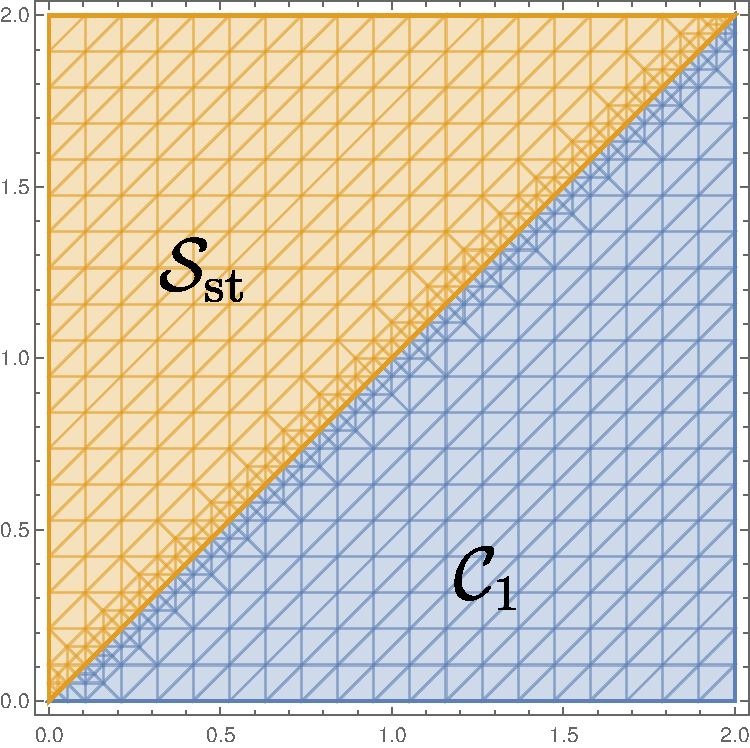
\includegraphics[width=0.3\textwidth]{Chaptersig/media/idealsfreelinear.pdf}}\label{fig.ideal.log}
  \hfill
  \subfloat[$\cSt$ and $\cC_{2}$.]{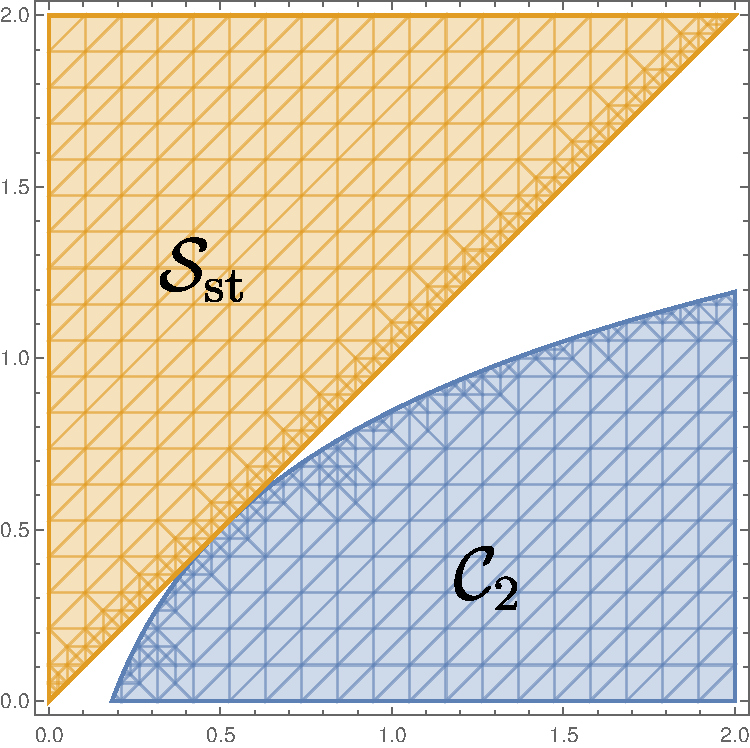
\includegraphics[width=0.3\textwidth]{Chaptersig/media/idealsfreelog.pdf}}\label{fig.ideal.power}
\hfill
  \subfloat[$\cSt$ and $\cC_{3}$.]{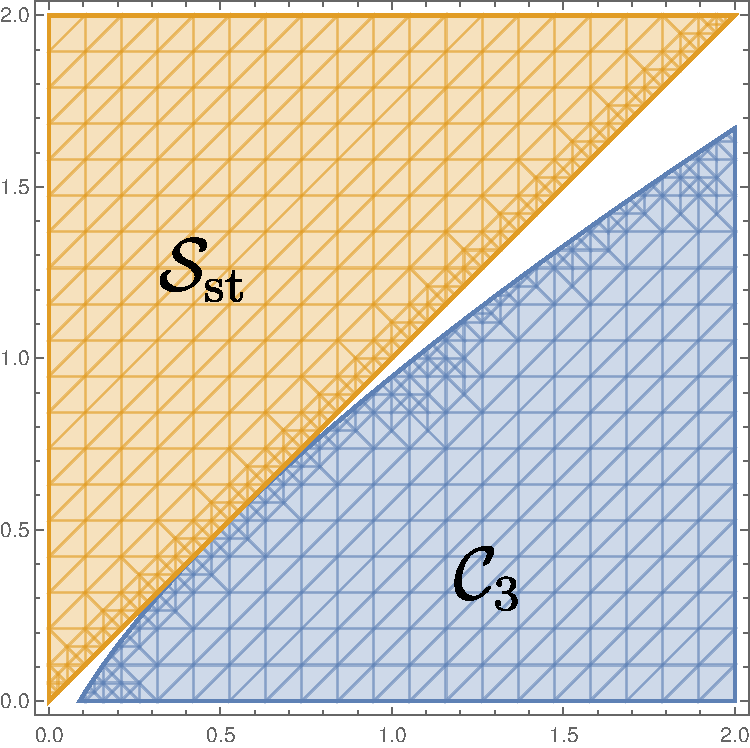
\includegraphics[width=0.3\textwidth]{Chaptersig/media/idealsfreepower.pdf}}\label{fig.exmpl.linear}
  \caption{$\cSt$-free sets.}
  \label{fig.ideal}
\end{figure}

\begin{example}
Consider the  hypograph of signomial term $x_1^{-2} x_2^{2}$ and
$
	\cSt = \{(x,y) \in \bR_{+}^3: y \le x_1^{-2} x_2^{2} \}.
$ For $(x,y) \in \bR_{++}^3$, $y \le x_1^{-2} x_2^{2}$ if and only if $ y^{1/3}x_1^{2/3} \le x_2^{2/3}$.  The following set is maximal $\cSt$-free in $\cG = \bR_+^3$:
$
	\cC_4 \deq \{(x,y) \in \bR_{+}^3:   y^{1/3}x_1^{2/3} \ge  \relx{x}_2^{2/3} + \frac{2}{3} \relx{x}_2^{-1/3} (x_2 - \relx{x}_2)\},
$
where $\relx{x}_2 \in \bR_{++}$. See \Cref{fig.free1} for $\relx{x}_2 = 0.2$.
\end{example}

\begin{example}
Consider the epigraph of signomial term $x_1^3 x_2$ and
$
	\cSt = \{(x,y) \in \bR_{+}^3: y \ge x_1^3 x_2\}.
$ For $(x,y) \in \bR_{++}^3$, $  y \ge x_1^3 x_2 $ if and only if $ y^{1/4} \ge x_1^{3/4}x_2^{1/4} $. The following set is maximal $\cSt$-free in $\cG = \bR_+^3$:
$
	\cC_5\deq \{(x,y) \in \bR_{+}^3:  \relx{y}^{1/4} + \frac{1}{4} \relx{y}^{-3/4}(y - \relx{y})\le x_1^{3/4}x_2^{1/4}  \},
$
where $\relx{y} \in \bR_{++}$. See \Cref{fig.free2} for $\relx{y} = 0.2$.
\end{example}
\begin{figure}[!ht]
 \centering
  \begin{subfigure}[b]{0.35\textwidth}
     	\centering
     	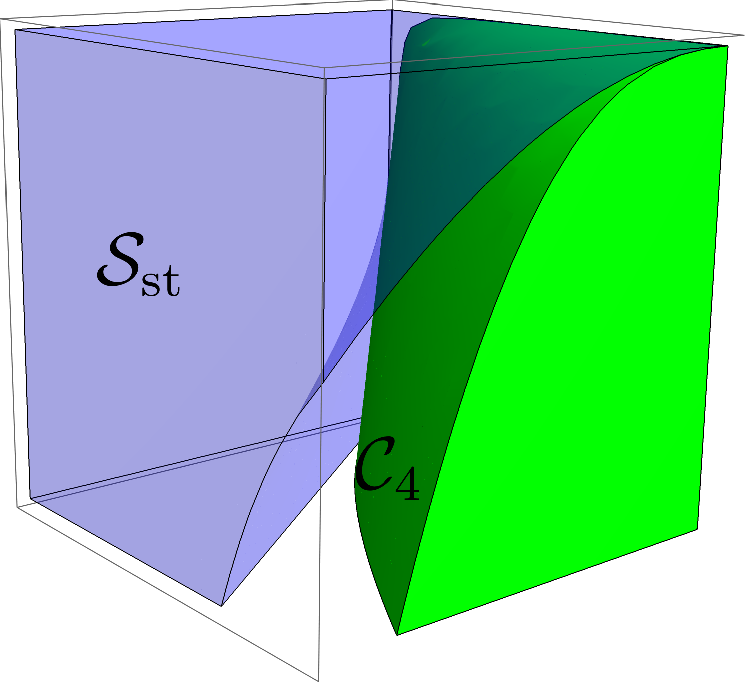
\includegraphics[width=\textwidth]{Chaptersig/media/sfree1.pdf}
     	\caption{$\cSt$ and $\cC_4$.}
    	\label{fig.free1}
 \end{subfigure}
 \hfill
  \begin{subfigure}[b]{0.35\textwidth}
     	\centering
     	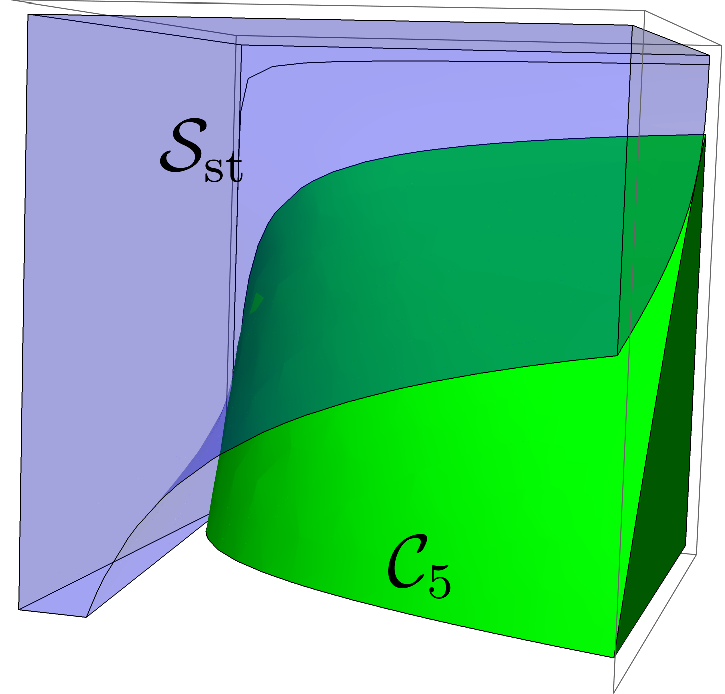
\includegraphics[width=\textwidth]{Chaptersig/media/sfree2.pdf}
     	\caption{$\cSt$ and $\cC_5$.}
    	\label{fig.free2}
 \end{subfigure}
  \caption{Two examples of $\cSt$ and $\cSt$-free sets.}
  \label{fig.free}
\end{figure}

 

\subsection{Computing intersection cuts}
\label{sec.sepic}
We focus on the separation of intersection cuts for the extended formulation of SP. In \Cref{sec.premic}, we presented a method to construct a simplicial cone $\cR$ from an LP relaxation. The vertex of that cone is  a relaxation solution $\relx{z} = (\relx{x}, \relx{y})$.

We assume that the LP relaxation includes all the linear constraints from \eqref{minlp2}. If $\relx{z}$ is not feasible for  \eqref{minlp2}, then $\relx{z}$ does not belong to the signomial lift. Hence, there exists a signomial term $g_i$ such that $\relx{y}_i \neq g_i(\relx{x})$. Given the reduced form $g'_i$,  we obtain a signomial term set $\cSt$: if $g_i(\relx{x}) > \relx{y}_i$, we choose $\cSt$ as the epigraph of $g'_i$; otherwise, we select it as the hypograph of $g'_i$.  This signomial term set yields a signomial-term-free set $\cC$ in \eqref{eq.sigfree} containing  $(\relx{u},\relx{v})$  in its interior (\Cref{cor.dc2}).  By applying the orthogonal lifting, we can transform $\cC$ into a signomial-lift-free set $\bar{\cC}$ as stated in  \Cref{cor.maxsig}.

We next show how to construct an intersection cut in \eqref{eq.ic}. It suffices to compute  step lengths $\eta^\ast_j$ in \eqref{eq.iccoef} along extreme rays $r^j$ of $\cR$. Each step length $\eta^\ast_j$ corresponds to a boundary point $\relx{z}+ \eta^\ast_j r^j$ in $\bd(\bar{\cC})$. The left-hand-side $\psi_{\beta}(u) - \lin{\psi_{\gamma}}{\relx{v}}(v)$  of the inequality in \eqref{eq.sigfree} is a concave function over $(u,v) \in \bR_{+}^h \times \bR^{\ell}$. Its  restriction along the ray $\relx{z}+ \eta_j r^j \;(\eta_j \in \bR_+)$ is a univariate concave function:
\begin{equation*}
 \tau_j:\bR_+ \to \bR, \eta_j \mapsto  \tau_j(\eta_j) \deq \psi_{\beta}(\relx{u} +  r^j_u \eta_j)  - \lin{\psi_{\gamma}}{\relx{v}}(\relx{v}+ r^j_v\eta_j),
\end{equation*}
where $r^j_u$ and $r^j_v$ are the projections of $r^j$ on $u$ and $v$ respectively. Let
$	\bar{\eta}_j \deq \sup_{\eta_j \ge 0}\{\eta_j:\relx{u} +  r^j_u \eta_j \ge 0\}$.
 Therefore, $\eta^\ast_j$ is the first point in $[0,\bar{\eta}_j]$  satisfying the boundary condition: either $ \tau_j(\eta^\ast_j) = 0$ or $\eta^\ast_j = \bar{\eta}_j$. Since  $\tau_j$ is a univariate concave function and $\tau_j(0) > 0$, there is at most one positive point in $\bR_+$ where $\tau_j$ is zero. We employ the bisection search method \cite{press2007chapter} to find such $\eta^\ast_j$.


 
 
 


\section{Convex outer approximation}
\label{sec.outerforsp}

In this section, we propose a convex nonlinear relaxation for the extended formulation \eqref{minlp3} of SP. This relaxation allows us to generate valid linear inequalities, known as outer approximation cuts, for SP. Unlike intersection cuts, outer approximation cuts do not require an LP relaxation \textit{a priori} .

Our goal is to construct a convex outer approximation of  the signomial lift. This gives rise to the convex nonlinear relaxation of SP.  To ensure the convergence of the sBB algorithm,  the feasible region of the extended formulation \eqref{minlp3} should be compact. 
Therefore, we assume that the signomial lift is in a hypercube. 

 Our algorithm approximates every signomial term set in the hypercube generated from the signomial lift. W.l.o.g., we consider a signomial term set in hypergraph or epigraph form. As \Cref{sec.siliftfree}, 
we can convert it in normalized DDC formulation:
\begin{equation}
\label{eq.st2}
	\cSt =  \{(u, v) \in \cU \times \cV:\, \psi_{\beta}(u) - \psi_{\gamma}(v) \le 0\},
\end{equation}
where $ \max(\lVert \beta \rVert_1, \lVert \gamma \rVert_1 ) = 1$, and $\cU,\cV$ are two hypercubes in $\bR_{+}^{h}, \bR_{+}^{\ell}$ respectively. The signomial term set is generally nonconvex, so we should find a convex outer approximation of $\cSt$.


Our construction involves convexifying the concave function $\psi_{\beta}$ in \eqref{eq.st2}. To do so, we will use the formal concepts of convex underestimators and convex envelopes.

Given a function  $f$ and a closed set $\cD \subseteq \bR^p$, a convex function $f':\conv(\cD) \to \bR$ is said to be a convex underestimator of $f$ over $\cD$, if, for all $x \in \cD$, $f'(x) \le f(x)$. The
 convex envelope $\conve_{\cD}(f)$  of $f$  is defined as the point-wise maximum convex underestimator of $f$ over $D$, \ie  $\epi(\conve_{\cD}(f)) = \conv(\epi_{\cD}(f))$, where $\epi_{\cD}(f) \deq \{(x,t) \in \cD \times \bR: f(x) \le t\}$.


 The following lemma gives an extended formulation of the convex envelope of a concave function over a polytope, where the formulation is uniquely determined by the function values at the vertices of the polytope. Based on \Cref{thm.poly}, we observe that the concave function $f$ is convex-extensible from its vertices (\ie $\conve_{P}(f)(x) = \conve_{Q}(f)(x)$ for $x \in P$), and $\conve_{P}(f)$ is a polyhedral function.



For the case of $P=\cU \deq \prod_{j \in [h]} [\underline{u}_j, \overline{u}_j]$ and $f =\psi_{\beta}$, $Q = \{q \in \bR^h: \forall j \in [h] \; q_j = \underline{u}_j \lor q_j = \overline{u}_j\}$ is the set of vertices of the hypercube $\cU$.  This yields an extended formulation of $\conve_{\cU}(\psi_{\beta})$. Replacing $\psi_{\beta}$ by its convex envelope $\conve_{\cU}(\psi_{\beta})$, we obtain a convex outer approximation of $ \cSt$ in \eqref{eq.st2}:
\begin{equation*}
\label{relcss}
  \bcSt\deq\{(u,v)\in \cU \times \cV: \conve_{\cU}(\psi_{\beta})(u) \le \psi_{\gamma}(v)\}.
\end{equation*}


By using this extended formulation, our convex nonlinear relaxation of SP incorporates additional auxiliary variables. Specifically, we require $2^h$ variables $\lambda_q$ to represent each convex envelope. For most SP problems in the \minlplib, where the degrees of signomial terms are less than 6, and $h$ is less than 3, the convex outer approximation remains computationally feasible.


\subsection{Outer approximation cuts}
To enhance efficiency, we propose a cutting plane algorithm to separate valid linear inequalities in the $(u,v)$-space from the extended formulation of the convex outer approximation. This algorithm generates a low-dimensional projection of $\bcSt$.



Given a point $(\relx{u}, \relx{v}) \in \cU \times \cV$, the algorithm determines whether it belongs to $\bcSt$. This verification can be done by checking the sign of $\conve_{\cU}(\psi_{\beta})(\relx{u}) - \psi_{\gamma}(\relx{v})$.  If $\conve_{\cU}(\psi_{\beta})(\relx{u}) - \psi_{\gamma}(\relx{v}) \le 0$, then $(\relx{u}, \relx{v}) \in \bcSt$. 

Since $\conve_{\cU}(\psi_{\beta})$ is a convex polyhedral function, our cutting plane algorithm evaluates the function by searching for an affine underestimator $a \cdot u+b$ of $\conve_{\cU}(u)$ such that $a \cdot \relx{u}+b = \conve_{\cU}(\relx{u})$. If $ (\relx{u}, \relx{v}) \notin \bcSt$, then   $a \cdot u+b \le  \psi_{\gamma}(\relx{v})$ is   a valid nonlinear inequality of $\bcSt$. Consequently, our cutting plane algorithm linearizes the inequality, resulting in  an outer approximation cut $a \cdot u+b \le  \lin{\psi_{\gamma}}{\relx{v}}(v)$: we recall that $\Xi$ is defined in Eq.~\eqref{def.Xi}.



 Due to \Cref{thm.poly}, we can solve the following LP to find the affine underestimator:
\begin{equation}
	\max_{a \in \bR^{h}, b \in \bR} a \cdot \relx{u}+b \quad \suc \forall q \in Q \; a \cdot q+b \le \psi_{\gamma}(q),
\end{equation}
where we omit the linear constraints that  bound $(a,b)$. The maximum value obtained from this LP  is exactly  $\conve_{\cU}(\psi_{\beta})(\relx{u})$. The affine underestimator $a \cdot \relx{u}+b$ is called a \emph{facet} of the envelope $\conve_{\cU}(\psi_{\beta})$, if $a \cdot \relx{u}+b \le t $ is a facet of $\epi(\conve_{\cU}(\psi_{\beta}))$. It should be noted that the solution of the LP is not necessarily a facet.


For $h = 1,2$, we can explicitly provide projected formulations of convex envelopes of power functions. This enables us to obtain facets of $\conve_{\cU}(\psi_{\beta})$ without the need to solve LPs. As a result, our cutting plane algorithm can efficiently separate outer approximation cuts for low-order problems.

To simplify our presentation, we translate and scale the domain of $\psi_{\beta}$ to $[0,1]^h$. This yields a new function $s(w) \deq \psi_{\beta}(u)$, where for all $j \in [h]$, $u_j \deq \overline{u}_j + (\overline{u}_j - \underline{u}_j)w_j$. After these transformations, we have $\cU = [0,1]^h$ and $Q = \{0,1\}^h$.   W.l.o.g., we focus on studying and computing facets of $\conve_{\cU}(s)$. For $h = 1$, the only facet is $s(0) + (s(1)- s(0))w_1$. 


 A set $D \subseteq \bR^h$ is called a \emph{product set}, if  $D = \bigtimes_{j \in [h]}D_j$ for $D_j \subseteq \bR$. Let $D$ be a product set. A function $f: D  \to \bR$ is \emph{supermodular} over $D$ (Section 2.6.1 of \cite{topkis2011supermodularity}), if the increasing difference condition holds:
for all $w^1,w^2 \in D, d \in \bR^h_{+}$ such that $w^1 \le w^2 $ and $ w^1+d, w^2+d \in D$, $f(w^1+d) -f(w^1)\le f(w^2 + d) -f(w^2)$. 
The following operations preserve supermodularity. 

\begin{lemma}
\label{lem.subtrans}
    Let $w' \in \bR^h, \rho \in \bR^h_{++}$,  and let $D'$ be a product subset of $D$. The following results hold: (restriction) $f$ is supermodular over $D'$;(translation) $ f(w+w')$ is supermodular over $D-d$; (scaling) $f(\rho * w)$ is supermodular over $D/\rho$, where $+, -, *, /$ are taken entry-wise.
\end{lemma}
\begin{proof}
    The results follow from the definition.
\end{proof}


 We note that when $D= Q$, $d$ is in $Q$.  We observe a useful property of $g$. 
 
\begin{proposition}
\label{lem.sup}
$s$ is supermodular over $Q$ and $\conve_{\cU}(s) = \conve_{\cQ}(g)$.
\end{proposition}
\begin{proof} 
According to Example 2.6.2 of \cite{topkis2011supermodularity}, the signomial term
$\psi_\alpha$ with $\alpha > 0$ is a Cobb-Douglas function, which is supermodular  over $\bR^h_{+}$. This implies that the power function $\psi_\beta$ is supermodular over $\bR^h_+$. By \Cref{lem.subtrans}, $s$ is supermodular over $\cU = [0,1]^h$. As $Q=\{0,1\}^h$ is a product subset of $\cU$,   $s$  is supermodular over $Q$. After the scaling and translation, $s$ is still concave, so it follows from \Cref{thm.poly} that $\conve_{\cU}(s) = \conve_{\cQ}(s)$.
\end{proof}

The search for facets of $s$ can be reduced to a more general problem, which involves finding facets of supermodular functions over  Boolean hypercubes.

We note that both power functions and multilinear terms can be considered Cobb-Douglas functions. Consequently, a similar argument can be used to demonstrate that multilinear terms are supermodular over any product subset of $\bR^h_+$.
  
\subsection{Convex envelopes of bivariate supermodular functions}

 
 Using the aforementioned result in \Cref{sec.conenvesuper}, we can construct an envelope-inducing family for bivariate supermodular functions. Let 
\begin{equation}
\label{eq.induce2}
    S^2_1 \deq \{00,10,01\}, S^2_2 \deq 
     \{11,10,01\}.
\end{equation}
One can find that $\conv(S^2_1)=\{(w_1,w_2) \in [0,1]^2:w_1 + w_2 \le 1 \}, \conv(S^2_2)=\{(w_1,w_2) \in [0,1]^2: w_1 + w_2 \ge 1 \}$ are two triangles in $[0,1]^2$.  We have that 
     	\begin{align*}
    	& f_{S^2_1}(w) =  f(00) + (f(10) -f(00)) w_1 + (f(01) -f(00)) w_2,\\
    	& f_{S^2_2}(w) = f(11) + (f(01) -f(11)) (1 - w_1) + (f(10) -f(11)) (1 - w_2).
	\end{align*}
 We show that these two affine functions define the convex envelope of $f$.
 
 \begin{theorem}
     For $h = 2$, $\{S^2_k\}_{k \in [2]}$ as in \eqref{eq.induce2}  is  envelope-inducing family in $Q$.
 \end{theorem}
 \begin{proof}
 It is easy to see that for all $k \in [2]$, $S^2_k$ is affinely independent and $\{\conv(S^2_k)\}_{k \in [2]}$ is a triangulation of $\cU$.  Therefore, it suffices to show that $\{S^2_k\}_{k \in [2]}$  is facet-inducing, \ie $f_{S^2_1}, f_{S^2_2}$ are affine underestimators of $f$. 
 
 \textbf{Case i.}
 We note that for all $w \in S^2_1 = \{00,10,01\}$, $f_{S^2_1}(w) = f(w).$ Note that $Q\smallsetminus S^2_1 = \{11\}.$ It follows from the definition of the affine function $f_{S^2_1}$  that
 \begin{equation*}
     f_{S^2_1}(11)= f_{S^2_1}(10) + (f_{S^2_1}(01) - f_{S^2_1}(00)) = f(10) + (f(01) - f(00)).
 \end{equation*}
 It follows from the supermodularity of $f$ that 
 \begin{equation*}
     f(10) + (f(01) - f(00)) \le  f(10) + (f(11) - f(10)) = f(11).
 \end{equation*}
 Thereby, $f_{S^2_1}$ underestimates $f$.

  \textbf{Case ii.}
 We note that for all $w \in S^2_2 = \{11,10,01\}$, $f_{S^2_2}(w) = f(w).$  Note that $Q\smallsetminus S^2_2 = \{00\}.$ It follows from the definition of the affine function $f_{S^2_2}$  that
 \begin{equation*}
     f_{S^2_2}(00)= f_{S^2_2}(10) - (f_{S^2_1}(11) - f_{S^2_1}(01)) = f(10) + (f(11) - f(01)).
 \end{equation*}
 It follows from the supermodularity of $f$ that 
 \begin{equation*}
     f(10) - (f(11) - f(01)) \le  f(10) - (f(10) - f(00)) = f(00),
 \end{equation*}
which concludes the proof.
 \end{proof}



 \subsection{Convexity and reverse-convexity}
 \label{sec.conv}
Our cutting algorithm can detect the convexity/reverse-convexity of signomial term sets. The detection is simply through  normalized  DDC formulations.

Denote by $e^\ell_j$ and $e^h_j$ the $j$-th unit vector in $\bR^h$ and $\bR^\ell$ respectively. Then, we have the following observations:
\begin{enumerate}
	\item[i)] if $\norm{\beta}_1 = 1,\gamma = 0$, \ie $\psi_{\beta}$ is concave and $\psi_{\gamma}$ is 1, then $\cSt$ is reverse-convex;
	\item[ii)] if $\norm{\beta}_1 \le 1,\gamma = e^\ell_j$ for some $j \in [\ell]$, \ie $\psi_{\beta}$ is concave and $\psi_{\gamma}$ is a linear univariate function, then $\cSt$ is reverse-convex;
   \item[iii)] if $\beta = e^h_j, \norm{\gamma}_1 \le 1$ for some $j \in [h]$, \ie
$\psi_{\beta}$ is a linear univariate function and $\psi_{\gamma}$ is concave, then  $\cSt$ is convex;
   \item[iv)] if $\norm{\beta}_1 = 0, \norm{\gamma}_1 = 1$, \ie $\psi_{\beta}$ is 1  and $\psi_{\gamma}$ is concave, then $\cSt$ is convex.
\end{enumerate}

We note that similar results are found in \cite{chen2009note,maranas1995finding}. The results in  \cite{chen2009note} are proved by checking the negative/positive-semidefiniteness of the Hessian matrix of a signomial term. According to the normalized DCC formulation, the results are evident.



\section{Computational results}
\label{sec.comp}


In this section, we conduct computational experiments to assess the efficiency of the proposed valid inequalities.



The \minlplib dataset comprises instances of MINLP problems that involve signomial terms, and some of these instances are SP problems. To build our benchmark, we select instances from \minlplib that satisfy the following criteria: (i) the instance includes signomial functions or polynomial functions, (ii) the continuous relaxation of the instance is non-convex. Our benchmark consists of a diverse set of 251 instances in which nonlinear functions consist of signomial and other functions. These problems frequently arise in practical applications and are commonly solved by general-purpose solvers.

Experiments are conducted on a server with  Intel Xeon W-2245 CPU @ 3.90GHz, 126GB main memory, and Ubuntu 18.04 system.  We use \scip 8.0.3 \cite{bestuzheva2023global}  as the framework for reading and solving problems, as well as conducting cut separation. \scip is integrated with \texttt{CPLEX} 22.1 as LP solver and \texttt{IPOPT} 3.14.7 as  NLP solver.


We evaluate the efficiency of the proposed valid inequalities in four different settings. The first setting, denoted as \disable, does not apply any of the proposed valid inequalities. The second setting, denoted as \oc, applies only the outer approximation cuts. The third setting, denoted as \ic, applies only the intersection cuts. The fourth setting combines both the \oc and \ic settings by applying both cuts.  We let \scip's default internal cuts to handle univariate signomial terms and multilinear terms. Our valid inequalities only handle the other high-order signomial terms.  The source code, data, and detailed results can be found in our online repository: \href{https://github.com/lidingxu/ESPCuts}{github.com/lidingxu/ESPCuts}.


In our benchmark, there are 150 instances classified as \emph{affected}, in which at least one of the \oc, \ic, and \oic settings adds cuts. There are 86 instances among the affected ones, for which \scip's default configuration (\ie the \disable setting) runs at least 500 seconds. Such instances are classified as \emph{affected-hard}. Each test run uses \scip configured by a setting to solve an instance. To solve the instances, we use the \scip solver with its sBB algorithm, imposing a time limit of 3600 seconds. For each test run, we measure the running time, the number of sBB search nodes, and the relative open duality gap.


To aggregate the performance metrics for a given setting, we compute shifted geometric means (SGMs) over our test set. The SGM for the running time incorporates a shift of 1 second. The SGM for the node number incorporates a shift of 100 nodes. The SGM for the relative gap incorporates a shift of 1$\%$. We  also compute SGMs of   performance metrics over the subset of affected and affected-hard instances. The performance results are presented in  \Cref{tb.perf}, where we also compute the relative values of SGMs of  performance metrics compared to the \disable setting. Our following analysis is based on the results on affected and affected-hard instances.





\begin{table} [htbp]
\centering
\resizebox{\columnwidth}{!}{
\addtolength{\tabcolsep}{-0.28em}
\begin{tabular}{cc|*{4}{c}|*{4}{c}|*{4}{c}}
\toprule
\multicolumn{2}{c|}{\multirow{2}{*}{Setting}}  &
\multicolumn{4}{c|}{All}    &
\multicolumn{4}{c|}{Affected} &
\multicolumn{4}{c}{Affected-hard}  \\
& &
{solved} &
{nodes}     &
{time} &
{gap}     &
{solved} &
{nodes}     &
{time} &
{gap}   &
{solved} &
{nodes}     &
{time} &
{gap}   \\
\midrule
\multirow{2}{*}{\disable} & absolute  & \multirow{2}{*}{138/251} &  6510.5 & 122.0 & 4.7\%  & \multirow{2}{*}{71/150} &  15592.4 & 253.6 & 5.7\% & \multirow{2}{*}{7/86} & 175973.8 & 3600.0 & 26.7\%  \\ 
 & relative &  & 1.0 & 1.0 & 1.0 & & 1.0 & 1.0 & 1.0 & & 1.0 & 1.0 & 1.0 \\
 \midrule
\multirow{2}{*}{\oc} & absolute  & \multirow{2}{*}{140/251}  &  5954.1 & 118.0 & 4.5\%  & \multirow{2}{*}{73/150} & 13443.9 & 241.4 & 5.4\% &  \multirow{2}{*}{10/86} & 115262.3 & 2872.7 & 23.3\%   \\ 
 & relative &  &    0.91 & 0.97 & 0.97 & & 0.86 & 0.95 & 0.95 & & 0.65 & 0.8 & 0.87 \\
 \midrule
 \multirow{2}{*}{\ic} & absolute  & \multirow{2}{*}{140/251} & 6144.3 & 122.4 & 4.4\% & \multirow{2}{*}{73/150} &  14081.5 & 252.1 & 5.2\% & \multirow{2}{*}{10/86} & 128072.7 & 2994.1 & 22.0\%  \\ 
 & relative &  & 0.94 & 1.0 & 0.95 & &  0.9 & 0.99 & 0.91 &  & 0.73 & 0.83 & 0.82\\
 \midrule
 \multirow{2}{*}{\oic} & absolute  & \multirow{2}{*}{139/251} &  5934.6 & 117.7 & 4.6\% &  \multirow{2}{*}{72/150} & 13275.6 & 236.8 & 5.6\% & \multirow{2}{*}{10/86}  & 118054.1 & 2758.3 & 23.0\%\\ 
 & relative &  &  0.91 & 0.96 & 0.99 & & 0.85 & 0.93 & 0.98 &  & 0.67 & 0.77 & 0.86\\
\bottomrule
\end{tabular}
}
\caption{Summary of performance metrics on \minlplib instances}\label{tb.perf}
\end{table}





First, we observe that  the proposed valid inequalities lead to the successful solution of 2 additional instances compared to the \disable setting. Considering the \oc setting, it solves 2 more instances than the \disable setting. Note that, in the affected-hard  benchmark, the number of solved instances by any non-disable setting is 3 more than that by the disable setting; in the affected  benchmark, the number of solved instances by any non-disable setting is at most 2 more than that by the disable setting. This is because restriction of the benchmark can reduces more solvable instances by the disable setting. 

The reductions in the running time, and relative gap achieved by the  \oc setting are  respectively  5\%, 5\% for affected instances and  20\%, 13\% for affected-hard instances. For the \ic setting, it solves 2 more instances than the \disable setting. The reductions in the running time, and relative gap achieved by the \ic setting are  respectively  1\%, 9\% for affected instances and 17\%, 14\% for affected-hard instances. In the case of the \oic setting, it solves 1 additional instance compared to  the \disable setting. The reductions in the running time, and relative gap achieved by the \oic setting are respectivel 7\%,  2\% for affected instances and  23\%, 14\% for affected-hard instances.

We note that the running time  does not give much information on affected-hard instances, because only 10 instances can be solved within 3600 seconds. For these instances, the gap reduction is more useful to measure the reduction of the search space by the proposed valid inequalities. However, for all affected instances, the running time  is still important, as it measures the acceleration by the valid inequalities. 

Secondly, we observe that all cut settings have a positive impact on the performance of \scip, although the extent of reduction varies. When comparing the \oc and \ic settings, we find that the \oc setting leads to a greater reduction in running time. This difference in running time arises because computing intersection cuts involves extracting a simplicial cone from the LP relaxation and applying bisection search along each ray of the cone. These procedures require more computational resources compared to the construction of outer approximation cuts.


On the other hand, the \ic setting demonstrates better performance in terms of gap reduction. Intersection cuts approximate the intersection of a signomial term set with the simplicial cone, while outer approximation cuts approximate the intersection of a signomial term set with a hypercube. Around the relaxation point, the simplicial cone typically provides a better  approximation than the hypercube. Hence, \ic achieves a larger reduction in the relative gap. However, the better simplicial conic approximation does yield a significant improvement compared to the hypercubic approximation.

Lastly, the \oic setting combines both the \oc and \ic settings, achieving the best reduction in the running time. However, for affected and affected-hard instances, the setting exhibits different results on gap reduction. In fact, the results of 
affected-hard instances give more insights, since the goal of valid inequalities is to accelerate the convergence for had instances. In this sense, the \oic setting achieves nearly the best result,  so it inherits the best of both valid inequalities.  However, its improvement compared to the individual settings is not significant.

To summarize, the performances of  the \oc and \ic settings are comparable. They can lead to smaller duality gap with less computational time, which are desirable for solvers, and one can use any of them. Moreover,  they do not hurt each other.



\section{Conclusion}

In this chapter, we study valid inequalities for SP problems, and propose two types of valid linear inequalities: intersection cuts and outer approximation cuts.  They are both derived from the normalized DCC formulations of signomial term sets. First, we study general conditions on maximal $\cS$-free sets. We construct maximal signomial-term-free sets, from which we  generate   intersection cuts. Secondly, we construct  convex outer approximations of signomial term sets within hypercubes. We provide extended formulations for the convex envelopes of the concave functions in the normalized DCC formulations. Then we separate valid inequalities for the convex outer approximations through projection.  Additionally, when $h=2$, we use supermodularity to derive a closed-form expression for the convex envelopes.
 

We present a comparative analysis of computational results obtained from the \minlplib instances. This analysis demonstrates the effectiveness of the proposed valid inequalities. The results indicate that intersection cuts and outer approximation cuts exhibit similar performance, and their combination inherits the best of the individual settings. In particular, it is straightforward to  implement outer approximation cuts in general-purpose solvers.  In the future, we intend to carefully fine-tune outer approximation cuts  and develop it as an easy-to-use plugin. 

We currently deal with signomial terms that explicitly present in the signomial lift, but our results can be extended to handle more ``faces'' of the signomial lift. In the future, the proposed valid inequalities can  approximate nonlinear aggregations of  constraints defining the signomial lift. Specifically, given signomial constraints $\{\psi_{\alpha^i}(x) = y_i\}_{i \in [r]}$, with  any exponent vector $\zeta \in \bR^r$, we can employ \emph{signomial aggregation} to generate a new signomial constraint: $\psi_{(\sum_{i \in [r]}\zeta_i\alpha^i)}(x) = \psi_{\zeta}(y)$. This constraint is valid for the signomial lift and encodes more variables and terms. Subsequently, we can apply DCC reformulation to the constraints  $\psi_{(\sum_{i \in [r]}\zeta_i\alpha^i)}(x) \le \psi_{\zeta}(y)$ and $\psi_{(\sum_{i \in [r]}\zeta_i\alpha^i)}(x) \ge \psi_{\zeta}(y)$. Finally, we can separate the proposed valid inequalities. As far as we know, the signomial aggregation operator is not used yet for polynomial programming, as it outputs a signomial constraint.




% ===============================================
% ===============================================




































